\newpage
\section{Personajes}

% ==============================================================================

\subsection{Ingeniera}

\textbf{Rol:} Daño a distancia

\begin{figure}[H]
	\centering
	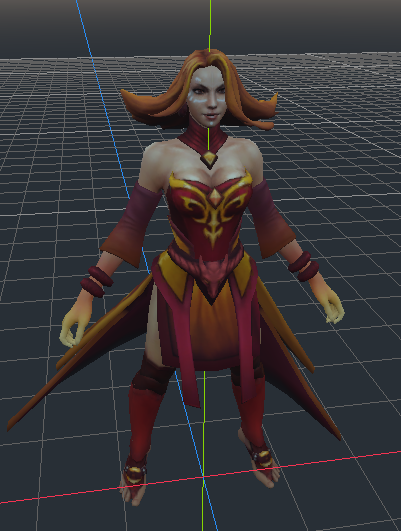
\includegraphics[width=0.4\linewidth]{figures/EngineerModel.png}
	% \caption{Ingeniera.}
	\label{fig:EngineerModel}
\end{figure}


La Ingeniera es un personaje que se especializa en el ataque a larga distancia mediante diversos tipos de proyectiles, aportando gran cantidad de daño a costa de tener poca vida y movilidad.

Para ser efectivo con ella, es importante mantener la distancia con los enemigos. Como la ingeniera solo tiene la $W$ para escapar del peligro, sus habilidades requieren que se quede inmóvil para usarlas y tiene poca vida, todo esto hace que sus opciones de supervivencia sean muy limitadas si los enemigos consiguen cubrir la distancia que los separa. 
% De esta forma, el gameplay de la ingeniera consiste en alejarse de los enemigos, atacarlos desde un lugar seguro y repetir este proceso cada vez que los enemigos consiguen acercarse.

\subsubsection{Habilidades}
\begin{itemize}
\item \textbf{Ataque Básico.} Dispara con una ballesta. El disparo hace poco daño pero tiene bastante rango. Es la única habilidad que no necesita que se quede quieta para usarse.
\item \textbf{Q.} Saca una pistola y dispara un proyectil de alcance infinito pero que no atraviesa obstáculos.
\item \textbf{W.} Dispara un gancho de alcance medio que, al impactar con un obstáculo, lleva a la ingeniera hasta este.
\item \textbf{E.} Dispara una granada que rebota con los obstáculos un número limitado de veces antes de explotar. 
% Tras chocar con un enemigo o alcanzarse el número máximo de rebotes, la granada explota, infringiendo daño en un área pequeña. 
El número máximo de granadas que puede haber en un momento dado en el mapa es de 3.
\item \textbf{Ultimate (R).} Saca una pistola gigante que tiene un tiempo de carga de 4 segundos antes de poderse usar. La pistola permite realizar 10 disparos en rápida sucesión con alcance ilimitado y que atraviesan todos los obstáculos y enemigos, causando daño moderado. Mientras la habilidad esté activa, la Ingeniera no puede realizar otra acción, pero la habilidad se puede cancelar en cualquier momento.
% Durante todo el proceso que dure la habilidad, la ingeniera no puede moverse del sitio. Si recibe crowd control (CC) durante el tiempo de carga o de uso de la habilidad, la habilidad se cancela, con lo que puede volver a moverse. También puede elegir cancelar la habilidad en cualquier momento de carga o uso. Al cancelarse, la carga de la ulti vuelve a 0. Esta habilidad tiene un CD largo.
\end{itemize}

% --------------------------------------------------------------

\subsection{Mago}
\textbf{Rol:} Apoyo / Tanque

\begin{figure}[H]
	\centering
	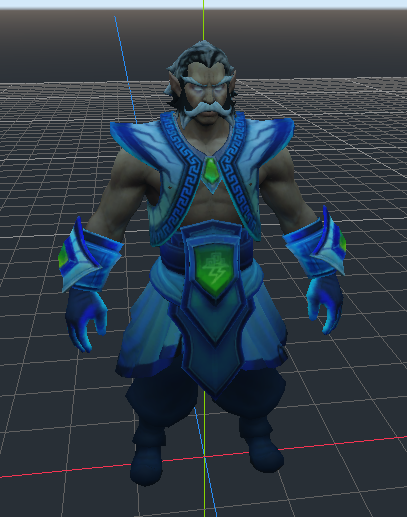
\includegraphics[width=0.4\linewidth]{figures/MageModel.png}
	% \caption{Mago}
	\label{fig:MageModel}
\end{figure}


El mago es un personaje de apoyo que se especializa en el control del mapa, proporcionando protección a su aliado y evitando que los enemigos puedan llegar hasta él. Sus características de \emph{tanque} le permiten preocuparse menos por su seguridad centrándose casi por completo en mantener a su aliado vivo y en darle apoyo.

Sus habilidades giran entorno al control del mapa y al posicionamiento de los distintos jugadores: él, su aliado y el equipo enemigo. Debe mantener alejado a su aliado del equipo enemigo, de ahí que tenga especial sinergia con campeones frágiles y/o con poca movilidad que tienen ataques a larga distancia. Su posicionamiento, en cambio, debe ser totalmente opuesto. Debido a sus habilidades y a su gran aguante, debe intentar siempre ``estar en medio'' del equipo enemigo, molestándolos e impidiéndoles llegar hasta su aliado.

\subsubsection{Habilidades}
\begin{itemize}
\item \textbf{Ataque Básico.} Da un golpe con su bastón. Este ataque, de corto alcance, hace muy poco daño pero invoca al hielo para aplicar una ralentización pequeña durante un periodo de tiempo.
\item \textbf{Q.} Invoca un elemento al azar sobre una zona. Los enemigos que pasen sobre esa zona recibirán un debuff que dependerá del tipo de elemento. De la misma forma, los proyectiles aliados que pasen sobre esa zona aplicarán el mismo debuff al impactar. Los elementos y sus debuffs asociados son: hielo - ralentización, fuego - daño por segundo, veneno - vulnerabilidad (aumenta el daño recibido por los siguientes ataques).
\item \textbf{W.} Intercambia su posición por la de su aliado.
\item \textbf{E.} Levanta un muro de piedra en la posición deseada.
\item \textbf{Ultimate (R).} Tras un largo tiempo de casteo (no cancelable) invoca a una tormenta que \emph{stunea} durante 5 segundos a los enemigos en una zona alrededor suya.
\end{itemize}

\newpage